% Fig. 2: answer structure -> guaranteed repair -> residual limit -> direct estimation.
% All numeric values are illustrative. Projection is not a CAPE stage.
\documentclass[11pt]{article}
\usepackage[paperwidth=16cm,paperheight=6.7cm,margin=0pt]{geometry}
\usepackage{amsmath,tikz}
\usepackage{unicode-math}
\setmainfont{Times New Roman}
\setmathfont{texgyretermes-math.otf}
\setmathrm{Times New Roman}
\usetikzlibrary{arrows.meta,calc}
\definecolor{cape}{HTML}{2F5DA8}
\definecolor{answer}{HTML}{B8DCD4}
\definecolor{answeralt}{HTML}{F1CCAA}
\definecolor{quiet}{HTML}{EAECEF}
\tikzset{
  >={Stealth[length=1.5mm,width=1.1mm]},
  flow/.style={->,draw=black!65,line width=.75pt,rounded corners=3pt},
  learned/.style={->,draw=cape,line width=.9pt,rounded corners=3pt},
  label/.style={font=\fontsize{10.95}{12.6}\selectfont,inner sep=0pt},
  heading/.style={label,font=\fontsize{10.95}{12.6}\selectfont\bfseries,anchor=west},
  score/.style={label,minimum width=6mm,minimum height=4.5mm,rounded corners=1pt},
  op/.style={label,align=center,draw=black!55,line width=.7pt,fill=white,
    rounded corners=2pt,minimum width=2.2cm,minimum height=1.1cm,inner sep=3pt},
}
\begin{document}
\pagestyle{empty}\noindent
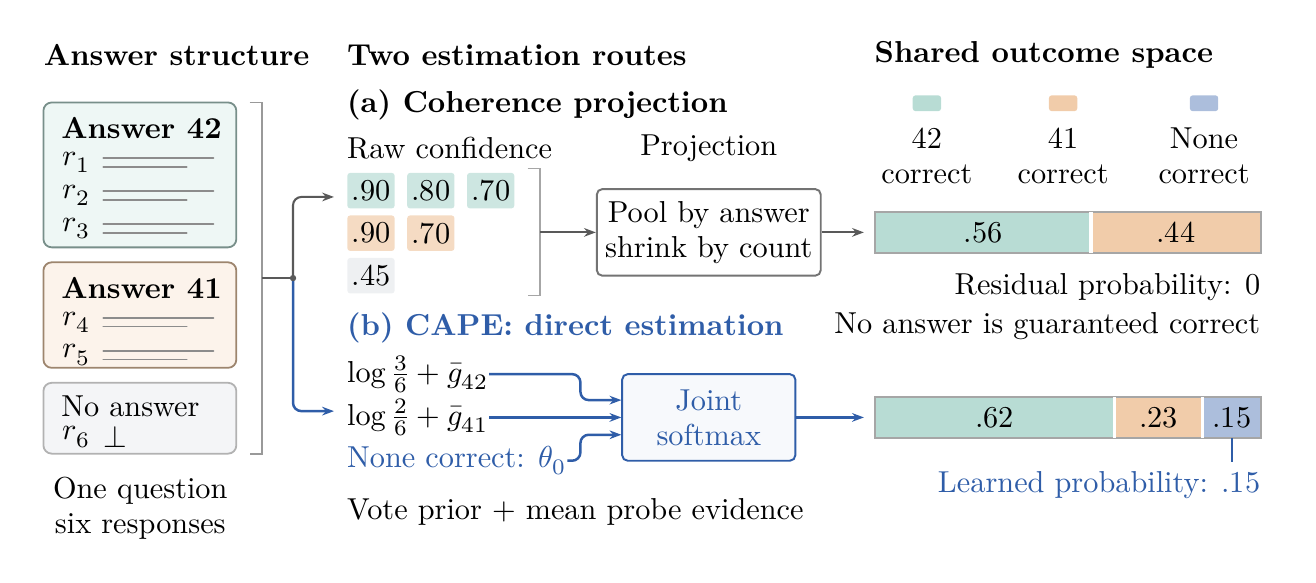
\begin{tikzpicture}[x=1cm,y=1cm,font=\fontsize{10.95}{12.6}\selectfont,text=black]
\path[use as bounding box] (0,0) rectangle (16,6.7);
\node[heading] at (.20,6.35) {Answer structure};
\node[heading] at (4.05,6.35) {Two estimation routes};
\node[heading] at (10.75,6.35) {Shared outcome space};

% One common input. Response IDs and answer identities persist across routes.
\draw[fill=answer!24,draw=answer!65!black,line width=.65pt,rounded corners=3pt]
  (.20,3.91) rectangle (2.65,5.75);
\node[heading] at (.42,5.43) {Answer 42};
\foreach \y/\i in {4.99/1,4.57/2,4.15/3}{
  \node[label,anchor=west] at (.44,\y) {$r_\i$};
  \draw[black!45,line width=.65pt,line cap=round] (.96,\y+.055)--(2.36,\y+.055)
    (.96,\y-.055)--(2.02,\y-.055);
}
\draw[fill=answeralt!24,draw=answeralt!65!black,line width=.65pt,rounded corners=3pt]
  (.20,2.38) rectangle (2.65,3.72);
\node[heading] at (.42,3.40) {Answer 41};
\foreach \y/\i in {2.96/4,2.54/5}{
  \node[label,anchor=west] at (.44,\y) {$r_\i$};
  \draw[black!45,line width=.65pt,line cap=round] (.96,\y+.055)--(2.36,\y+.055)
    (.96,\y-.055)--(2.02,\y-.055);
}
\draw[fill=quiet!50,draw=black!30,line width=.65pt,rounded corners=3pt]
  (.20,1.29) rectangle (2.65,2.19);
\node[label,anchor=west] at (.42,1.89) {No answer};
\node[label,anchor=west] at (.44,1.50) {$r_6$};
\node[label,anchor=west] at (.96,1.50) {$\bot$};
\node[label,align=center] at (1.43,.60) {One question\\six responses};

% A single bracket and fork convey the shared grouping input.
\draw[black!40,line width=.7pt] (2.82,5.75)--(2.98,5.75)--(2.98,1.29)--(2.82,1.29);
\draw[black!65,line width=.75pt] (2.98,3.52)--(3.37,3.52);
\draw[flow] (3.37,3.52)--(3.37,4.55)--(3.89,4.55);
\draw[learned] (3.37,3.52)--(3.37,1.83)--(3.89,1.83);
\fill[black!65] (3.37,3.52) circle (1.15pt);

% Upper route: repair arbitrary existing response scores.
\node[heading] at (4.05,5.72) {(a) Coherence projection};
\node[label,anchor=west] at (4.05,5.17) {Raw confidence};
\foreach \x/\v in {4.36/.90,5.12/.80,5.88/.70}{
  \node[score,fill=answer!70] at (\x,4.63) {$\v$};
}
\foreach \x/\v in {4.36/.90,5.12/.70}{
  \node[score,fill=answeralt!70] at (\x,4.09) {$\v$};
}
\node[score,fill=quiet!80] at (4.36,3.55) {$ .45 $};
\draw[black!35,line width=.6pt] (6.35,4.91)--(6.51,4.91)--(6.51,3.30)--(6.35,3.30);
\node[op,minimum width=2.65cm] (project) at (8.65,4.10) {Pool by answer\\shrink by count};
\draw[flow] (6.51,4.10)--(project.west);
\node[label] at (8.65,5.17) {Projection};
\draw[flow] (project.east)--(10.62,4.10);

% Lower route: direct learning from vote priors and cluster-mean evidence.
\node[heading,text=cape] at (4.05,2.89) {(b) CAPE: direct estimation};
\node[label,anchor=west] (logit42) at (4.05,2.30)
  {$\log\frac{3}{6}+\bar g_{42}$};
\node[label,anchor=west] (logit41) at (4.05,1.75)
  {$\log\frac{2}{6}+\bar g_{41}$};
\node[label,anchor=west,text=cape] (null) at (4.05,1.20) {None correct: $\theta_0$};
\node[op,draw=cape,fill=cape!4,text=cape] (softmax) at (8.65,1.75) {Joint\\softmax};
\draw[learned] (logit42.east)--(7.02,2.30)--(7.02,1.97)--(7.54,1.97);
\draw[learned] (logit41.east)--(7.54,1.75);
\draw[learned] (null.east)--(7.02,1.20)--(7.02,1.53)--(7.54,1.53);
\draw[learned] (softmax.east)--(10.62,1.75);
\node[label,anchor=west] at (4.05,.55) {Vote prior $+$ mean probe evidence};

% Shared outcome legend; stacked bars expose the single probability budget.
\foreach \x/\col/\name in {11.42/answer/{42\\correct},13.15/answeralt/{41\\correct},14.94/cape!40/{None\\correct}}{
  \fill[\col,rounded corners=1pt] (\x-.18,5.64) rectangle (\x+.18,5.84);
  \node[label,align=center] at (\x,5.07) {\name};
}
% Projection: answer masses exhaust the budget, so all-wrong mass is zero.
\fill[answer] (10.76,3.84) rectangle (13.504,4.36);
\fill[answeralt] (13.504,3.84) rectangle (15.66,4.36);
\draw[black!35,line width=.55pt] (10.76,3.84) rectangle (15.66,4.36);
\draw[white,line width=1.1pt] (13.504,3.84)--(13.504,4.36);
\node[label] at (12.132,4.10) {$ .56 $};
\node[label] at (14.582,4.10) {$ .44 $};
\node[label,anchor=east] at (15.66,3.40) {Residual probability: $0$};
\node[label,anchor=east] at (15.66,2.91) {No answer is guaranteed correct};
% CAPE: a directly learned distribution includes the outside option.
\fill[answer] (10.76,1.49) rectangle (13.798,2.01);
\fill[answeralt] (13.798,1.49) rectangle (14.925,2.01);
\fill[cape!40] (14.925,1.49) rectangle (15.66,2.01);
\draw[black!35,line width=.55pt] (10.76,1.49) rectangle (15.66,2.01);
\foreach \x in {13.798,14.925}{\draw[white,line width=1.1pt] (\x,1.49)--(\x,2.01);}
\node[label] at (12.279,1.75) {$ .62 $};
\node[label] at (14.3615,1.75) {$ .23 $};
\node[label] at (15.2925,1.75) {$ .15 $};
\draw[cape,line width=.65pt] (15.2925,1.49)--(15.2925,1.18);
\node[label,anchor=east,text=cape] at (15.66,.89) {Learned probability: $.15$};
\end{tikzpicture}
\end{document}
